\clearpage


\section{等待 ALOHA 的设计及分析}

经典时隙 ALOHA 以实现简单、分布式程度高而被广泛采用，但其接入决策主要围绕“是否发送”展开，并未区分不同终端状态信息的新鲜程度。在 AoI 约束下，这一处理方式存在明显不足：刚完成更新的终端仍可立即回到竞争过程，而未更新的终端却可能因长时间未接入信道，导致其在接收端的状态信息严重老化。为缓解这一问题，本章在传统 ALOHA 框架中引入成功传输后的确定性等待机制，构造一种面向信息时效性的等待 ALOHA 协议。

本章内容的安排如下，3.1 节先给出等待 ALOHA 的系统模型、AoI 演化规律以及退避规则，并说明为何后续分析可以归结为离开时间间隔 $Y$ 的统计刻画；3.2 节基于马尔可夫链建立稳态接入模型，推导碰撞概率的稳态方程，并讨论其解的存在性与唯一性；3.3 节在此基础上进一步推导平均 AoI 与 AoI 违规概率的闭式表达；3.4 节结合所得结果讨论等待窗口对系统性能的影响；3.5 节对本章工作进行总结。

\subsection{系统模型}

本章考虑一个由单个接入点（Access Point, AP）和 $N$ 个终端组成的无线网络，该网络采用时隙化 ALOHA 的接入方式，所有终端在公共信道上竞争传输机会。

在经典时隙 ALOHA 中，时间被划分为等长的离散时隙，每个终端在时隙的起始处以固定概率 $p_0$ 接入信道并发送数据。若同一时隙内存在两个及以上的终端同时发送，则认为发生碰撞，发送失败。为降低连续碰撞带来的信道拥塞，系统在传输失败后为发生碰撞的终端分配一个退避计时器。随着时隙推进，该计时器将逐时隙递减，只有当计时器减至零时，终端才能够重新接入信道。

在上述的随机接入框架下，本文进一步引入按需生成采样机制。与维护缓存队列的传统状态更新系统不同，终端仅在决定发起传输时才对物理过程进行采样，并立即生成新的状态更新包。因此，发送端的排队时延被完全消除。按照 AoI 的定义，任一终端在离散时隙 $t$ 的 AoI 演化可写为
\begin{equation}
    \label{eq:aoi_evolution}
    \Delta(t+1) =
    \begin{cases}
        1, & \text{若终端在时隙 } t \text{ 成功传输了状态更新包} \\
        \Delta(t) + 1, & \text{其他情况}
    \end{cases}
\end{equation}

经典时隙 ALOHA 的优势在于协议简单、控制开销低且易于分布式实现，因此在低负载、少终端场景下具有较好的适用性。然而，在面向大规模接入的状态更新系统中，接收端更关注各终端状态信息的新鲜程度。若某一终端刚完成更新，则接收端已经掌握了其最新状态；相比之下，那些长期未能成功接入的终端往往对应更高的 AoI，理应优先获得传输机会。从面向 AoI 的视角来看，所有终端围绕信道的竞争不应完全独立，而应体现一定程度的协同。

基于这一考虑，本文提出一种基于等待的随机接入机制，并将其引入时隙 ALOHA 中，构造等待 ALOHA 协议。其核心规则包括：

\textbf{（1）成功传输后的确定性等待。} 当终端成功完成一次状态更新后，协议强制其在接下来的 $z$ 个时隙内不参与信道竞争。参数 $z$ 为等待窗口长度，其作用是抑制刚完成更新的终端再次接入信道，让尚未完成更新的终端获得更多的传输机会。

\textbf{（2）碰撞后的随机退避。} 当终端发送失败时，仍沿用传统 ALOHA 中的随机退避机制，即生成服从 $\beta \sim \text{unif}(0,w-1)$ 的退避计时器，以降低后续时隙中重复碰撞的概率。

据此，终端 $i$ 在时隙 $t$ 的退避计时器满足
\begin{equation}
    b_i(t + 1) =
\begin{cases}
z, & \text{if } b_i(t) = 0, \, b_j(t) \neq 0 \ \forall j, \\
\beta, & \text{if } b_i(t) = 0, \, b_j(t) = 0 \ \exists j, \\
b_i(t) - 1, & \text{if } b_i(t) \neq 0.
\end{cases}
\end{equation}
式中，$b_j(t)$ 表示除终端 $i$ 之外的其他终端在 $t$ 时刻下的退避计时器状态。该机制下 AoI 的典型演化轨迹如图\ref{fig:cp3_aoi_evolution}所示：若在某一段时间内未收到终端的更新数据包，则 AoI 线性增长；一旦成功接收更新，AoI 立即下降到 1。
\begin{figure}[h]
\centering
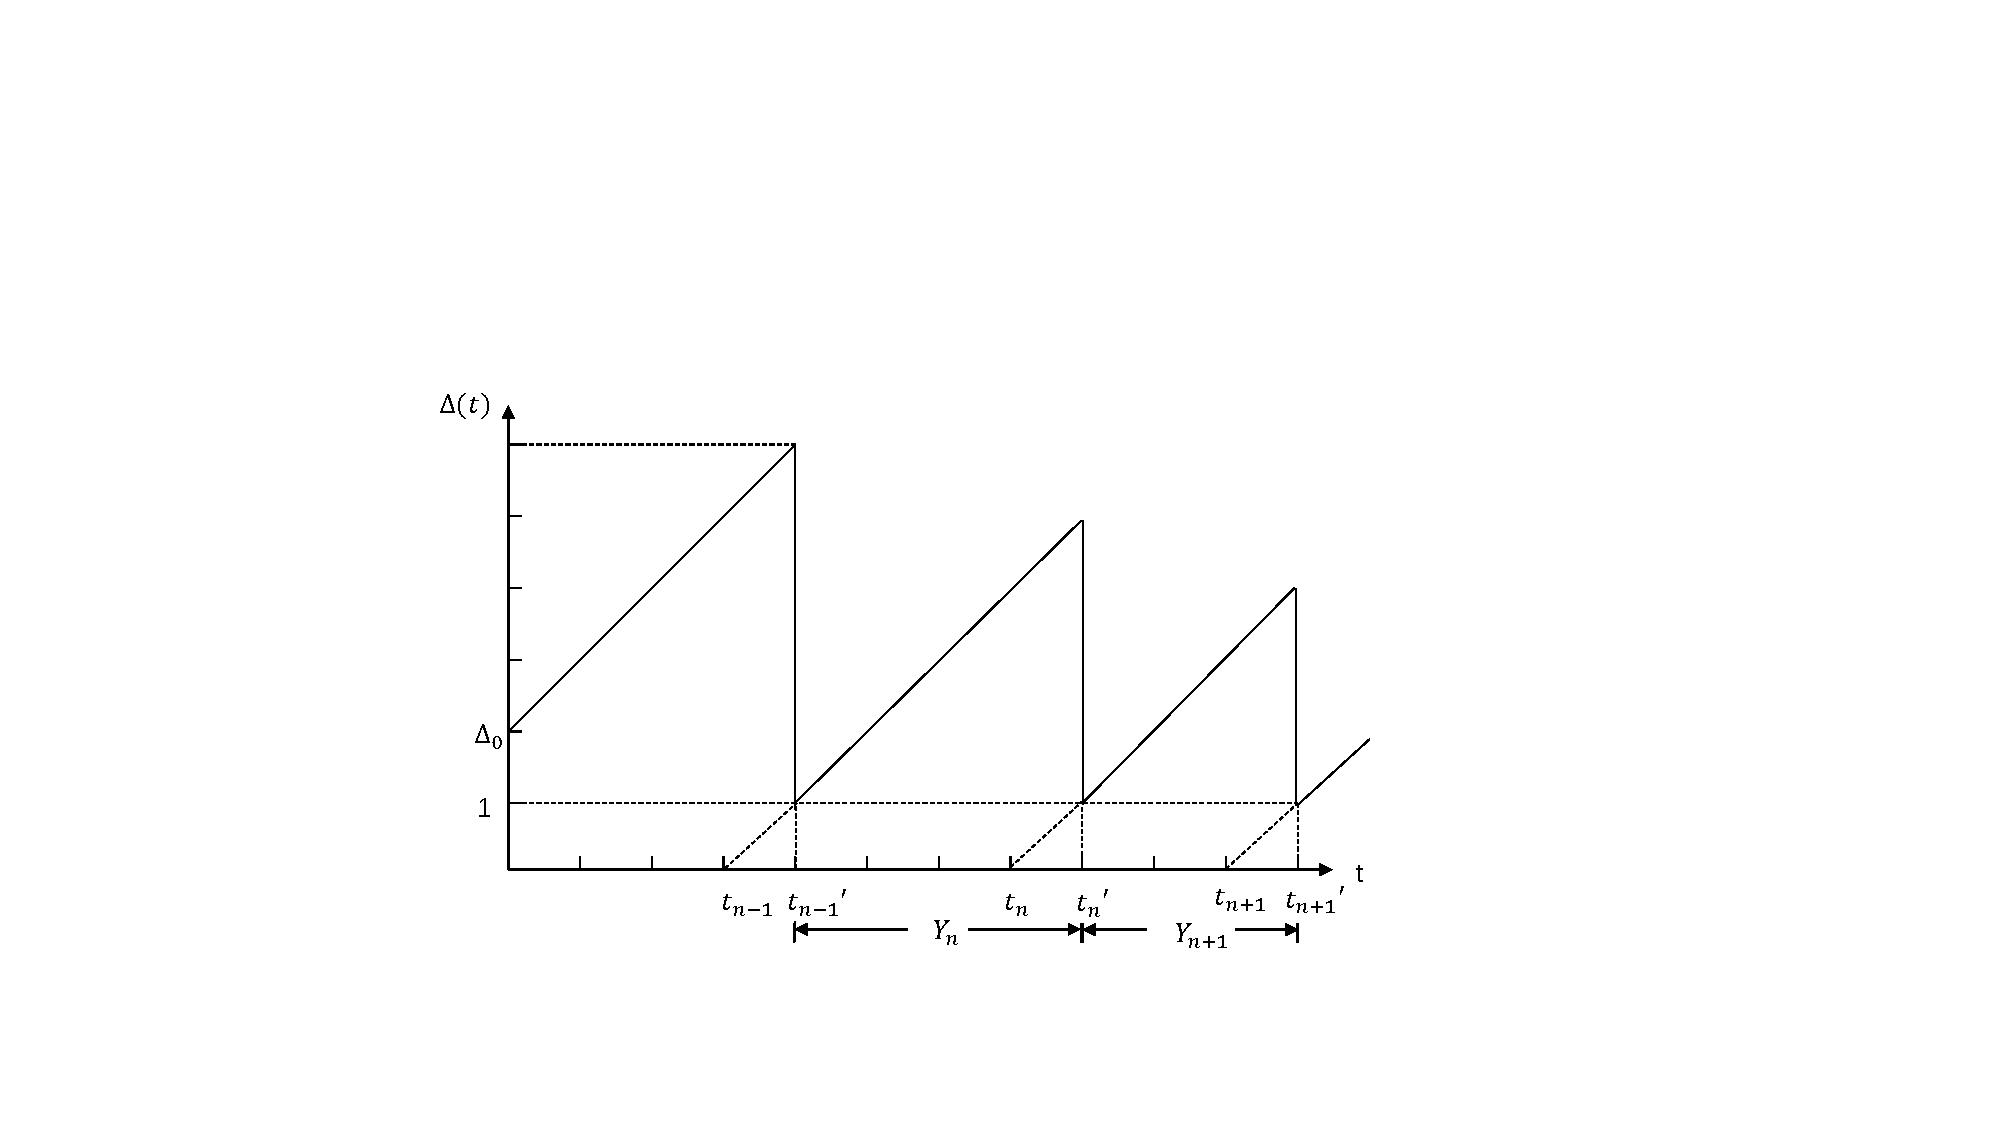
\includegraphics[width=0.8\textwidth]{figure/cp3/AoI演化趋势图.pdf}
\caption{AoI 演化趋势图}
\label{fig:cp3_aoi_evolution}
\end{figure}

由第二章给出的统一分析框架可知，平均 AoI 与 AoI 违规概率的计算均归结为求解相邻两次成功更新之间的离开时间间隔 $Y$ 的统计特性，即 $Y$ 的一阶矩和二阶矩。最直接的做法是对整个系统建立联合马尔可夫链，将所有终端的 AoI、退避计时器及终端的数量一并纳入状态空间。然而，当 $N$ 增大时，该联合状态空间会呈指数级膨胀，导致求解极为困难。

为此，本文借鉴 Bianchi 模型中的解耦思想，采用常见的稳态近似：当网络规模较大且系统进入稳态后，目标终端在任意时隙内感知到的碰撞概率 $p_{cl}$ 可以近似视为与时间无关的常数。换言之，当目标终端发起传输时，其他终端的状态分布已经稳定，其对目标终端形成的竞争环境在统计意义上保持不变。基于该近似，可以将原始的高维耦合系统降维为单个目标终端的离散时间马尔可夫链，为后续的解析推导奠定基础。

\subsection{基于马尔可夫链的稳态接入分析}

在等待 ALOHA 中，单次传输是否成功取决于其余终端是否在同一时隙内同时发送，因此稳态碰撞概率 $p_{cl}$ 是本章分析的核心参数。基于前述解耦假设，本节首先构造单个目标终端的离散时间马尔可夫链模型，随后建立发送概率与碰撞概率之间的稳态方程，并讨论解的存在性与唯一性。

\subsubsection{状态转移模型}

为刻画目标终端在等待 ALOHA 机制下的微观行为，记其在时隙 $t$ 的状态为 $(m(t),n(t))$，其中 $m(t)$ 表示当前退避计时器的取值，$n(t)$ 表示当前的 AoI。定义
\begin{equation}
    b_{i,k}=\lim_{t \to +\infty} \text{Pr}\{m(t)=i,n(t)=k\}
\end{equation}
为系统处于稳态时的状态概率。

当退避计时器大于 0 时，终端不参与信道竞争，因此经过一个时隙后，退避计时器减 1，而 AoI 则加 1。只有当退避计时器等于 0 时，终端才具备发包资格，此时存在以下三种状态转移：
\begin{enumerate}[wide]
    \item 终端保持静默，不发起传输。状态从 $(0,k)$ 转移到 $(0,k+1)$，转移概率为 $1-p_0$；
    \item 终端发起传输但发生碰撞。此时状态从 $(0,k)$ 转移到 $(i,k+1)$，其中 $i \in [0,w-1]$，转移概率为 $q=\frac{p_0 p_{cl}}{w}$；
    \item 终端成功发送更新包。此时 AoI 被重置为 1，退避计时器被置为 $z$，即状态从 $(0,k)$ 转移到 $(z,1)$，转移概率为 $p_s=p_0(1-p_{cl})$。
\end{enumerate}

由于成功发送后的终端必须等待 $z$ 个时隙，因此系统存在一条确定性的状态链
\[
(z,1)\to(z-1,2)\to\cdots\to(1,z)\to(0,z+1).
\]
这意味着在稳态下，终端重新进入可竞争状态时，其 AoI 必然不小于 $z+1$。基于上述转移规则，可以得到完整的二维马尔可夫链，如图\ref{fig:cp3_aloha_system_tran_photo}所示。为简化书写，令
\[
p=(1-p_0)+\frac{p_0p_{cl}}{w},
\]
并记 $\omega$ 为预设的 AoI 门限。
\begin{figure}[h]
    \centering
    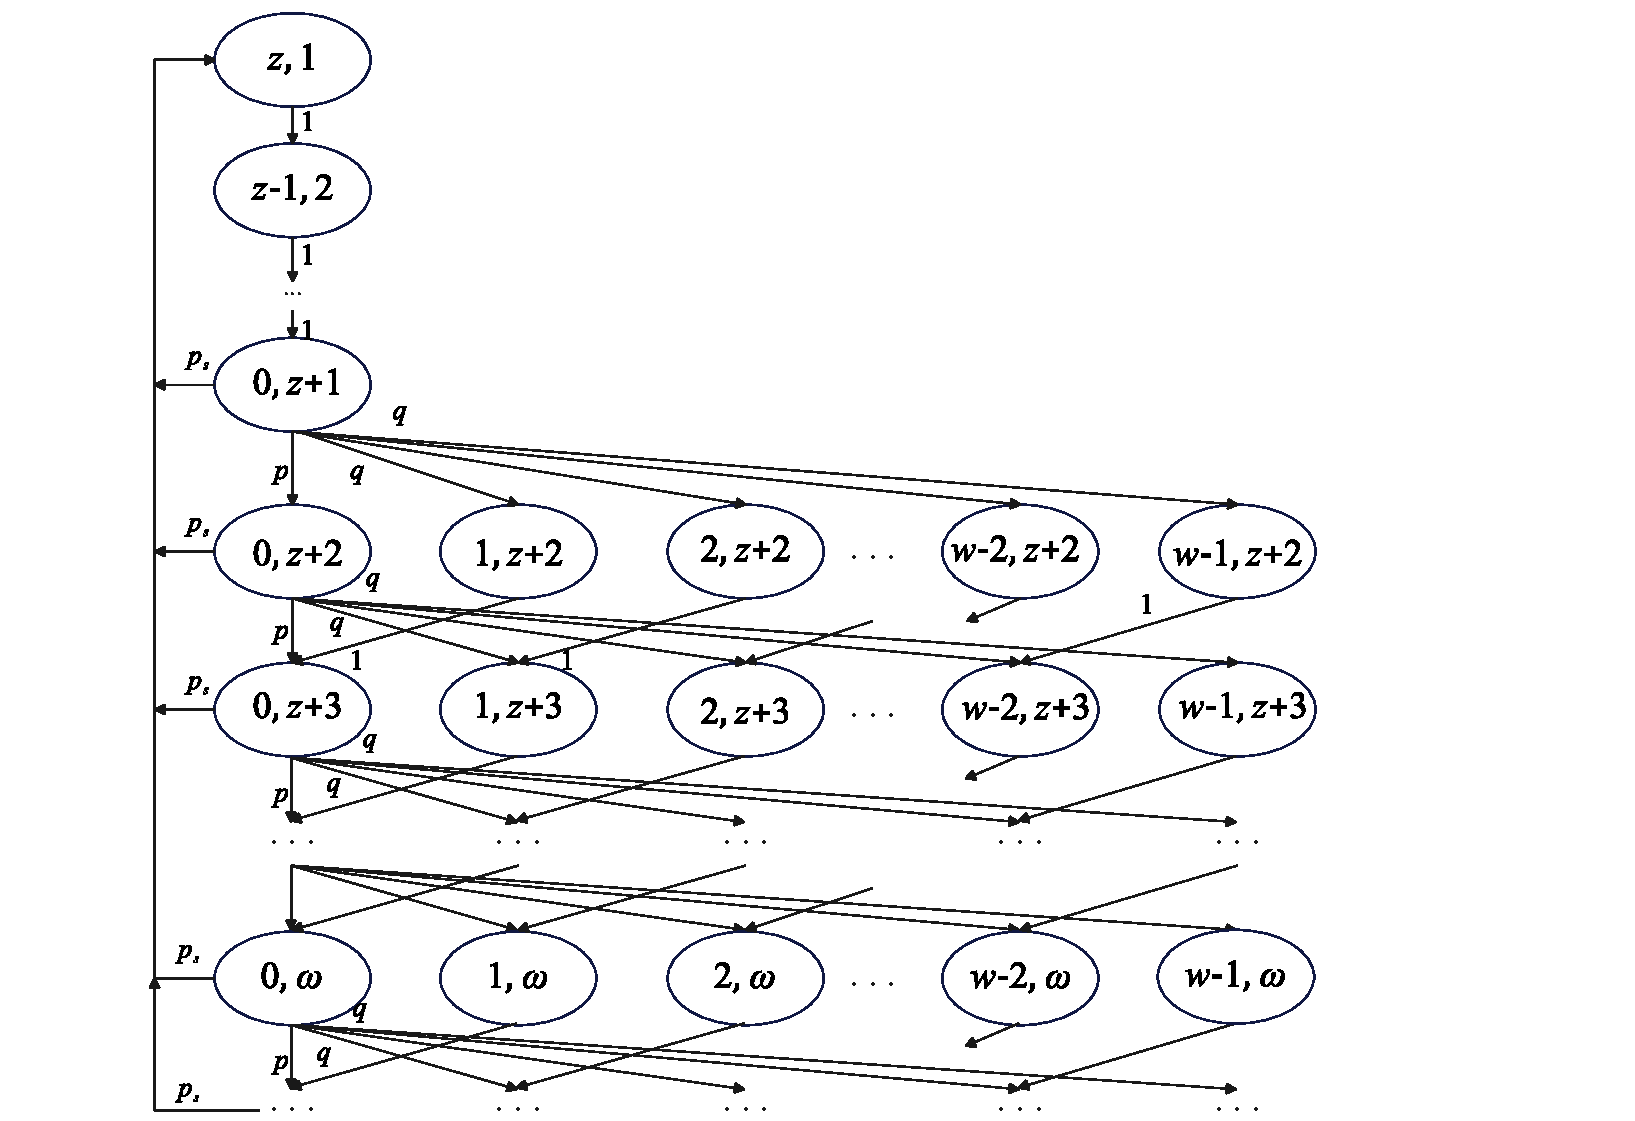
\includegraphics[width=1.2\textwidth]{figure/cp3/系统的状态转移图.pdf}
    \caption{系统的状态转移图}
    \label{fig:cp3_aloha_system_tran_photo}
\end{figure}

\subsubsection{稳态方程的构建}

根据图\ref{fig:cp3_aloha_system_tran_photo}的状态结构，任意状态 $(i,k)$ 的稳态概率均可表示为若干活跃状态概率 $b_{0,m}$ 的线性组合。首先，当 AoI 不超过 $z+1$ 时，所有这些状态都只能由一次成功传输触发，因此有
\begin{equation} \label{cp3_b_ik_aoi_le_z+1}
    b_{z,1}=b_{z-1,2}=b_{z-2,3}=\cdots=b_{0,z+1}=p_s\sum_{k=z+1}^{+\infty}b_{0,k}
\end{equation}

当 AoI 恰好等于 $z+2$ 时，有
\begin{equation}\label{cp3_b_ik_equal_z+2}
    b_{0,z+2} = pb_{0,z+1},\quad b_{i,z+2}=qb_{0,z+1},\quad1\leq i \leq w-1
\end{equation}

当 AoI 大于 $z+2$ 时，可进一步得到如下递推关系：
\begin{equation}\label{cp3_b_ik_great_z+2}
\begin{gathered}
\begin{cases}
    \displaystyle b_{0,n} = p b_{0,n-1} + q \sum_{k=z+1}^{n-2} b_{0,k}, & z+3 \le n \le z+w+1 \\[12pt]
    \displaystyle b_{0,n} = p b_{0,n-1} + q \sum_{k=n-w}^{n-2} b_{0,k}, & n > z+w+1 \\[12pt]
    \displaystyle b_{m,n} = q \sum_{k=z+1}^{n-1} b_{0,k}, & m \ge 1, \, m+n \le z+w+1 \\[12pt]
    \displaystyle b_{m,n} = q \sum_{k=m+n-w}^{n-1} b_{0,k}, & m \ge 1, \, m+n > z+w+1
\end{cases}
\end{gathered}
\end{equation}

利用概率的归一化条件，将式\eqref{cp3_b_ik_aoi_le_z+1}、式\eqref{cp3_b_ik_equal_z+2}与式\eqref{cp3_b_ik_great_z+2}联立，可得
\begin{equation}
\begin{split}
(z+1)p_0(1-p_{cl}) \sum_{k=z+1}^{\infty} b_{0,k} + (1-p_0) \sum_{k=z+1}^{\infty} b_{0,k} \\
+ p_0 p_{cl} \sum_{k=z+1}^{\infty} b_{0,k} + \frac{p_0 p_{cl}(w-1)}{2} \sum_{k=z+1}^{\infty} b_{0,k} = 1
\end{split}
\end{equation}
整理后得到
\begin{equation}\label{cp3_sum_of_b_0k}
\sum_{k=z+1}^{\infty} b_{0,k} = \frac{1}{1 + z p_0 - z p_0 p_{cl} + \frac{p_0 p_{cl} w}{2} - \frac{p_0 p_{cl}}{2}}
\end{equation}

式\eqref{cp3_sum_of_b_0k}表明，所有活跃状态概率的总和最终仅由稳态碰撞概率 $p_{cl}$ 决定。由于终端在任一时隙内发起传输的平均概率等于其处于活跃状态且选择发送的联合概率，因此有
\begin{equation}\label{cp3_avg_send_prob}
    \tau=p_0\sum_{k=z+1}^{+\infty}b_{0,k}=\frac{p_0}{1+zp_0+p_0p_{cl}(\frac{w-1}{2}-z)}=\tau(p_{cl})
\end{equation}

另一方面，在包含 $N$ 个终端的网络中，若假设各终端在稳态下的发送行为相互独立，则目标终端在一次发送中遭遇碰撞的概率为
\begin{equation}\label{cp3_pcl_with_tau}
    p_{cl} = 1- (1-\tau)^{N-1}
\end{equation}

将式\eqref{cp3_avg_send_prob}代入式\eqref{cp3_pcl_with_tau}，消去中间变量 $\tau$，即可得到关于 $p_{cl}$ 的稳态方程
\begin{equation}\label{cp3_pcl}
    p_{cl} = 1 - (1 - \tau(p_{cl}))^{N-1} \triangleq f(p_{cl})
\end{equation}
为了后续的性能分析，接下来将对该方程进行求解。

\subsubsection{稳态方程解的存在唯一性论证}

式\eqref{cp3_pcl}是一个非线性的方程，难以直接写出闭式解。因此，在使用数值求解之前，要先说明两个问题：其一，该方程在定义域 $[0,1]$ 上是否存在解；其二，在什么条件下该解是唯一的。为此，定义辅助函数
\begin{equation}
    F(x)=x-f(x), \qquad x\in[0,1]
\end{equation}
其中
\begin{equation}
    f(x)=1-\left(1-\tau(x)\right)^{N-1}, \qquad
    \tau(x)=\frac{p_0}{1+zp_0+p_0x\left(\frac{w-1}{2}-z\right)}.
\end{equation}

先讨论方程解的存在性。考察区间端点处的函数值，由 $\tau(0)=\frac{p_0}{1+zp_0}\in(0,1)$ 可得
\begin{equation}
    F(0)=-f(0)=-\left[1-\left(1-\frac{p_0}{1+zp_0}\right)^{N-1}\right]<0.
\end{equation}
另一方面，由于
\[
\tau(1)=\frac{p_0}{1+zp_0+p_0\left(\frac{w-1}{2}-z\right)}
=\frac{p_0}{1+\frac{p_0(w-1)}{2}}\in(0,1),
\]
因此
\begin{equation}
    F(1)=1-f(1)=\left(1-\tau(1)\right)^{N-1}>0.
\end{equation}
又因为 $\tau(x)$ 与 $f(x)$ 在闭区间 $[0,1]$ 上连续，所以 $F(x)$ 在 $[0,1]$ 上也连续。由介值定理可知，至少存在一个 $x^\star\in(0,1)$ 使得 $F(x^\star)=0$，即稳态方程\eqref{cp3_pcl}在 $[0,1]$ 上至少存在一个解。

进一步考察唯一性所需的单调性条件。记
\[
D(x)=1+zp_0+p_0x\left(\frac{w-1}{2}-z\right),
\]
则
\begin{equation}
    \tau'(x)= -\frac{p_0^2\left(\frac{w-1}{2}-z\right)}{[D(x)]^2}.
\end{equation}
由链式法则，
\begin{equation}
    f'(x)=(N-1)\left(1-\tau(x)\right)^{N-2}\tau'(x),
\end{equation}
从而
\begin{equation}
    F'(x)=1-f'(x)
    =1-(N-1)\left(1-\tau(x)\right)^{N-2}\tau'(x).
\end{equation}

注意到 $D(x)>0$ 对任意 $x\in[0,1]$ 恒成立，因此 $\tau'(x)$ 的符号完全由 $\frac{w-1}{2}-z$ 决定。这意味着等待窗口 $z$ 与随机退避窗口 $w$ 的相对大小，将直接影响 $f'(x)$ 的取值。

当 $w\ge 2z+1$ 时，有
\begin{equation}
    \frac{w-1}{2}\ge z,
\end{equation}
则有 $\tau'(x)\le 0$，于是
\begin{equation}
    f'(x)\le 0,\qquad x\in[0,1].
\end{equation}
也就是说，$f(x)$ 在 $[0,1]$ 上单调不增。由此立即得到
\begin{equation}
    F'(x)=1-f'(x)\ge 1>0,
\end{equation}
即 $F(x)$ 在 $[0,1]$ 上严格单调递增。

结合前述结论 $F(0)<0$ 与 $F(1)>0$，可知 $F(x)$ 只能与横轴相交一次，因此方程\eqref{cp3_pcl}在区间 $[0,1]$ 上存在唯一解。换言之，当随机退避窗口满足
\begin{equation}
    w\ge 2z+1
\end{equation}
时，等待 ALOHA 的稳态碰撞概率被唯一确定。

相对地，当 $w<2z+1$ 时，
\begin{equation}
    \frac{w-1}{2}<z,
\end{equation}
则 $\tau'(x)>0$，进而 $f'(x)>0$。此时 $f(x)$ 随 $x$ 增大而增大，$F'(x)=1-f'(x)$ 未必始终为正。虽然方程仍然因连续性而至少存在一个解，但仅凭上述分析已无法保证解的唯一性。特别是在网络规模 $N$ 较大时，因子 $(N-1)$ 会放大 $f'(x)$ 的数值，使得 $f'(x)$ 超过 1 的可能性显著增加，进而导致 $F(x)$ 失去单调性。因此，$w<2z+1$ 时不能直接推出唯一解的结论。

综上所述，在满足 $w\ge 2z+1$ 的条件下，函数 $F(x)$ 在 $[0,1]$ 上连续且严格递增，并满足 $F(0)<0<F(1)$。因此，二分法可以稳定求得唯一根 $p_{cl}^\star$，其步骤如下：
\begin{enumerate}[wide]
    \item \textbf{初始化：} 取左右端点 $l_0=0$、$r_0=1$，并给定收敛阈值 $\epsilon>0$；
    \item \textbf{区间折半：} 在第 $t$ 轮迭代中计算中点 $m_t=(l_t+r_t)/2$，并求取 $F(m_t)$；
    \item \textbf{区间更新：} 若 $F(m_t)=0$，则 $m_t$ 即为所求；若 $F(m_t)<0$，则令 $l_{t+1}=m_t,\ r_{t+1}=r_t$；否则令 $l_{t+1}=l_t,\ r_{t+1}=m_t$；
    \item \textbf{停止准则：} 当 $|r_t-l_t|<\epsilon$ 时停止迭代，并以区间中点作为 $p_{cl}^\star$ 的数值近似。
\end{enumerate}

\subsection{信息时效性指标的理论解析}
\subsubsection{平均 AoI 的闭式推导}

第二章已经给出了平均 AoI 的计算公式\eqref{cp2_avg_aoi}。由于本章系统中每个时隙的长度均为 1，故平均 AoI 的计算公式可重写为
\begin{equation}\label{cp3_avg_aoi}
    \Delta = 1 + \frac{E[Y^2]}{2E[Y]}
\end{equation}
其中，$Y$ 表示相邻两次成功更新之间的离开时间间隔。因此，平均 AoI 的闭式推导可归结为求解随机变量 $Y$ 的一阶矩和二阶矩。

\begin{enumerate}[wide]
    \item 求解 $Y$ 的一阶矩

    设在一个离开时间间隔 $Y$ 内，终端共发起 $\alpha$ 次传输尝试。由于在解耦假设下，每次尝试的碰撞概率均为常数 $p_{cl}$，因此 $\alpha$ 服从参数为 $1-p_{cl}$ 的几何分布，其概率质量函数为
    \begin{equation}\label{cp3_alpha_expression}
        \Pr\{\alpha=k\}=(1-p_{cl})p_{cl}^{k-1},\quad k=1,2,\dots
    \end{equation}

    根据等待 ALOHA 的工作机制，一次完整的离开时间间隔由三部分组成：成功更新后等待 $z$ 个时隙、每次发送前的接入等待，以及每次碰撞后的随机退避。设单次接入前的等待时隙数为 $I$，则
    \begin{equation}\label{cp3_I_expression}
        \Pr\{I=i\}=(1-p_0)^{i-1}p_0
    \end{equation}

    终端前 $k-1$ 次发送均碰撞，第 $k$ 次发送成功，将对应的离开时间间隔记为 $Y_k$，有
    \begin{equation}\label{cp3_Yk_expression}
        Y_k=z+\sum_{j=1}^{k-1}(I_j+\beta_j)+I_k
        =z+\sum_{j=1}^{k}I_j+\sum_{j=1}^{k-1}\beta_j
    \end{equation}
    其中，$\beta_j$ 表示第 $j$ 次碰撞后的随机退避计时器。

    由于各个 $I_j$ 与 $\beta_j$ 相互独立，且同分布，因此
    \begin{equation}\label{cp3_EYk}
        E[Y_k]=z+\frac{k}{p_0}+\frac{(k-1)(w-1)}{2}
    \end{equation}

    将式\eqref{cp3_alpha_expression}与式\eqref{cp3_EYk}联立，可得
    \begin{equation}\label{cp3_EY}
        \begin{split}
            E[Y] &= \sum_{k=1}^{+\infty}\Pr\{\alpha=k\}E[Y_k] \\
            &= z\sum_{k=1}^{+\infty}(1-p_{cl})p_{cl}^{k-1} + \frac{1}{p_0}\sum_{k=1}^{+\infty}k(1-p_{cl})p_{cl}^{k-1} \\
            &\quad + \frac{w-1}{2}\sum_{k=1}^{+\infty}(k-1)(1-p_{cl})p_{cl}^{k-1} \\
            &= z + \frac{1}{p_0(1-p_{cl})} + \frac{p_{cl}(w-1)}{2(1-p_{cl})}
        \end{split}
    \end{equation}

    \item 求解 $Y$ 的二阶矩

    对于给定的 $\alpha=k$，有
    \begin{equation}\label{cp3_EYk^2}
        E[Y_k^2] = D(Y_k) + (E[Y_k])^2
    \end{equation}

    根据方差的线性性质以及独立性，有
    \begin{equation}\label{cp3_DYk}
        D(Y_k) = \sum_{j=1}^{k} D(I_j) + \sum_{j=1}^{k-1} D(\beta_j) = k D(I) + (k-1) D(\beta)
    \end{equation}

    将式\eqref{cp3_DYk}、式\eqref{cp3_EYk}和式\eqref{cp3_EYk^2}联立，得到
    \begin{equation}\label{cp3_EYK^2_withAB}
        \begin{aligned}
            E[Y_k^2] &= k \frac{1-p_0}{p_0^2} + (k-1)\frac{w^2-1}{12} + (U + kV)^2 \\
            &= \left( U^2 - \frac{w^2-1}{12} \right) + k \left[ \frac{1-p_0}{p_0^2} + \frac{w^2-1}{12} + 2UV \right] + k^2 V^2
        \end{aligned}
    \end{equation}
    其中，
    \[
    U=z-\frac{w-1}{2},\qquad V=\frac{1}{p_0}+\frac{w-1}{2}.
    \]

    与式\eqref{cp3_alpha_expression}联立，最终得到
    \begin{equation}\label{cp3_EY2}
        \begin{aligned}
            E[Y^2] &= \sum_{k=1}^{+\infty} \Pr\{\alpha=k\} E[Y_k^2] \\
            &= \left( U^2 - \frac{w^2-1}{12} \right) \sum_{k=1}^{+\infty}(1-p_{cl})p_{cl}^{k-1} \\
            &\quad + \left[ 2UV + \frac{1-p_0}{p_0^2} + \frac{w^2-1}{12} \right] \sum_{k=1}^{+\infty} k(1-p_{cl})p_{cl}^{k-1} \\
            &\quad + V^2 \sum_{k=1}^{+\infty} k^2(1-p_{cl})p_{cl}^{k-1}
        \end{aligned}
    \end{equation}
    整理后得到
    \begin{equation}\label{cp3_EY2result}
        E[Y^2] = z^2 + \left[ \frac{2 + p_{cl} p_0 (w-1)}{p_0 (1-p_{cl})} \right] z + C_0
    \end{equation}
    其中
    \begin{equation*}
        \begin{split}
            C_0 &= \frac{1}{(1-p_{cl})^2} \Bigg\{ \frac{p_{cl}(p_{cl}+2)}{6} w^2 - \frac{p_{cl} [ p_0(1+p_{cl}) - 4 ]}{2 p_0} w \\
                &\quad + \frac{p_{cl}(2p_{cl}+1)}{6} - \frac{p_{cl}+1}{p_0} + \frac{2}{p_0^2} \Bigg\}
        \end{split}
    \end{equation*}
\end{enumerate}

最后，将式\eqref{cp3_EY}、式\eqref{cp3_EY2result}与式\eqref{cp3_avg_aoi}联立即可得到平均 AoI 的闭式表达式
\begin{equation}\label{cp3_AoI_Final}
    \begin{aligned}
        \Delta = 1 + \frac{z^2 + \left[ \frac{2 + p_{cl} p_0 (w-1)}{p_0 (1-p_{cl})} \right] z + C_0}{2 \left[ z + \frac{1}{p_0(1-p_{cl})} + \frac{p_{cl}(w-1)}{2(1-p_{cl})} \right]}
    \end{aligned}
\end{equation}


\subsubsection{AoI 违规概率的闭式推导}

图\ref{fig:cp3_aoi_evolution_with limit}给出了门限为 $\omega$ 时的 AoI 演化示意图。根据第二章中 AoI 违规概率的计算公式\eqref{cp2_aoi_violation_expression}，在本章模型下，求解违规概率的关键在于求解违规量 $J=\max(0,1+Y-\omega)$ 的期望，即 $E[J]$。
\begin{figure}[h]
    \centering
    
\includegraphics[width=0.8\textwidth]{figure/cp3/有限制的AoI演化图.pdf}
    \caption{具有 $\omega$ 限制的 AoI 演化图}
    \label{fig:cp3_aoi_evolution_with limit}
\end{figure}

从构成上来看，$Y$ 由几何分布控制的重传次数、几何分布的接入等待以及均匀分布的退避时长共同叠加而成。原则上通过卷积可以获得其精确分布，但相应的表达式将会是分段且难以用于后续解析的复杂形式。为兼顾物理的可解释性与计算的可操作性，本文采用矩匹配方法对 $Y$ 的分布进行近似。

考虑到 $Y$ 必然取正值，且在碰撞与退避作用下通常呈现右偏和长尾的特征，因此采用移位指数分布作为近似模型更为自然。设
\[
Y\sim c+\mathrm{Exp}(\lambda),
\]
则其概率密度函数为
\begin{equation} \label{cp3_fy}
    f_Y(y; c, \lambda) = \lambda e^{-\lambda(y-c)}, \quad y \ge c
\end{equation}
其中，$c\ge0$ 为位置参数，用于描述成功更新后强制等待带来的最小时延下界；$\lambda>0$ 为尺度参数，用于刻画尾部的衰减速度。

根据移位指数分布的统计特性，有
\begin{equation}
    E[Y] = c + \frac{1}{\lambda},\quad D[Y] = E[Y^2] - (E[Y])^2 = \frac{1}{\lambda^2}
\end{equation}
联立式\eqref{cp3_EY}和式\eqref{cp3_EY2result}，可解得
\begin{equation}\label{cp3_lambdaandc}
    c = E[Y] - \frac{1}{\lambda} = E[Y] - \sqrt{D[Y]},\quad \lambda = \frac{1}{\sqrt{D[Y]}}
\end{equation}

由图\ref{fig:cp3_aoi_evolution_with limit}可知，峰值 AoI 为 $1+Y$，故违规量为
\[
J=\max(0,1+Y-\omega).
\]
记 $H=\omega-1$，则
\begin{equation}\label{cp3_EJ}
\begin{aligned}
    E[J] &= E[\max(0, Y - H)] = \int_{H}^{\infty} (y - H) f_Y(y; c, \lambda) dy \\
    &= \int_{H}^{\infty} (y-H)\lambda e^{-\lambda(y-c)}dy
\end{aligned}
\end{equation}
化简可得
\begin{equation}
    E[J]  = \frac{1}{\lambda} e^{-\lambda(H-c)}
\end{equation}
与式\eqref{cp3_lambdaandc}联立，得到
\begin{equation}\label{cp3_EJresult}
    E[J] = \sqrt{D[Y]} \exp\left( -\frac{\omega - 1 - \mathbb{E}[Y]}{\sqrt{D[Y]}} - 1 \right)
\end{equation}

再将式\eqref{cp3_EJresult}与式\eqref{cp3_EY}一起代入计算公式\eqref{cp2_aoi_violation_expression}，最终得到 AoI 违规概率的闭式表达式
\begin{equation}\label{cp3_violation_prob_simplified}
    \Pr\{\Delta(t) > \omega\} = \frac{\sqrt{C_0 - M^2}}{z + M} \exp\left( -\frac{\omega - 1 - (z + M)}{\sqrt{C_0 - M^2}} - 1 \right)
\end{equation}
其中
\begin{equation}\label{cp3_M}
    M = \frac{2 + p_{cl} p_0 (w-1)}{2 p_0 (1-p_{cl})}
\end{equation}

\subsection{理论分析与性能洞察}

在得到平均 AoI 与 AoI 违规概率的闭式表达式后，本节将进一步讨论等待 ALOHA 的性能表现。为简化书写，记
\[
\mu_Y = E[Y] = z + M,\qquad \sigma_Y^2 = D[Y] = C_0 - M^2.
\]
其中，$M$ 由式\eqref{cp3_M}给出。

\subsubsection{平均 AoI 的方差惩罚效应}

将 $\mu_Y$ 与 $\sigma_Y^2$ 代入式\eqref{cp3_AoI_Final}，可将平均 AoI 改写为
\begin{equation}\label{cp3_aoi_deconstructed}
    \Delta = 1 + \frac{\mu_Y^2 + \sigma_Y^2}{2\mu_Y} = 1 + \frac{\mu_Y}{2} + \frac{\sigma_Y^2}{2\mu_Y}
\end{equation}

式\eqref{cp3_aoi_deconstructed}将平均 AoI 分解为两个部分：
\begin{enumerate}[wide]
    \item $1 + \frac{\mu_Y}{2}$ 反映了平均离开时间间隔对 AoI 的基本影响；
    \item $\frac{\sigma_Y^2}{2\mu_Y}$ 反映了离开时间间隔波动带来的额外惩罚。
\end{enumerate}

这一定量分解表明，在 AoI 优化问题中，仅仅缩短平均离开时间间隔并不足够；若离开时间间隔伴随着较大的波动，平均 AoI 仍会显著恶化。等待 ALOHA 中引入的确定性等待窗口 $z$，本质上正是通过对刚完成更新的终端施加可控约束，以此来换取全网竞争强度的下降和离开时间间隔方差的收缩。对面向 AoI 的随机接入设计而言，这种“以确定性换稳定性”的思路是其区别于传统吞吐量导向设计的关键所在。

\subsubsection{违规概率的变异系数主导与尾部衰减规律}

将 $\mu_Y$ 与 $\sigma_Y$ 代入式\eqref{cp3_violation_prob_simplified}，可得
\begin{equation}\label{cp3_violation_deconstructed}
    \Pr\{\Delta(t) > \omega\} = \frac{\sigma_Y}{\mu_Y} \exp\left( -\frac{\omega - 1 - \mu_Y}{\sigma_Y} - 1 \right)
\end{equation}

该式揭示了两个重要结论：
\begin{enumerate}[wide]
    \item 系数 $\frac{\sigma_Y}{\mu_Y}$ 是离开时间间隔的变异系数，这个系数说明违规概率不仅取决于离开时间间隔的期望值，而且也受离开时间间隔离散程度的直接影响；
    \item 当门限 $\omega$ 大于 $1+\mu_Y$ 时，违规概率关于门限差值呈指数衰减，而衰减快慢由 $\sigma_Y$ 决定。$\sigma_Y$ 越大，尾部衰减越慢，极端陈旧状态出现的概率则越高。
\end{enumerate}

因此，等待 ALOHA 对违规概率的改进并不只体现为平均意义上的 AoI 降低，更体现在对尾部风险的抑制。特别是在高负载场景下，若不对竞争行为进行额外约束，碰撞引发的连续退避会迅速拉长右尾，导致 AoI 违规概率显著上升。

\subsubsection{确定性等待窗口 \texorpdfstring{$z$}{z} 的参数权衡效应}

在所提出的等待 ALOHA 中，参数 $z$ 是最关键的设计。增大 $z$ 会直接拉长成功更新后的等待时间，因此从单个终端视角看，它会增大平均离开时间间隔 $\mu_Y$。但从系统视角看，较大的 $z$ 意味着刚成功更新的终端将在后续的若干时隙中退出竞争，从而降低单位时隙内处于活跃状态的终端数，以此来缓解信道的碰撞。

因此，$z$ 的作用具有典型的权衡特征：一方面，它引入了额外的确定性等待开销；另一方面，它减少了随机碰撞带来的不确定性时延。对于终端规模较大的接入场景，后者往往更为重要，因为系统性能的主要恶化来源并不是固定等待本身，而是碰撞所诱发的长尾退避过程。适当增大 $z$，实质上是将一部分不可控的随机延迟转换为可控的确定性延迟，从而在整体上改善平均 AoI，并降低 AoI 违规风险。

\subsection{本章小结}

本章围绕等待 ALOHA 的设计与分析展开。针对经典时隙 ALOHA 无法区分不同终端时效需求的问题，本文在成功传输后引入确定性等待机制，建立了等待 ALOHA 的系统模型，并在按需生成采样假设下刻画了其 AoI 演化与退避行为。进一步地，借助解耦近似与马尔可夫链建模，本文给出了碰撞概率的稳态方程，并证明了在 $w\ge 2z+1$ 条件下该方程解的存在性与唯一性。

在此基础上，本章以离开时间间隔 $Y$ 为分析主线，推导了平均 AoI 与 AoI 违规概率的闭式表达，并从方差惩罚、尾部衰减以及等待窗口权衡等角度解释了等待机制改善信息时效性的原因。上述结果表明，适度限制刚完成更新终端的再次竞争，能够在增加可控等待的同时有效抑制碰撞引起的长尾效应，从而为后续章节对更复杂接入机制的讨论提供理论参照。
